\openingarticle
\def\ppages{\pagerange{NASC:firstpage}{NASC:lastpage}}
\def\shorttitle{Conference Review: National Archaeology Student Conference Australia}
\def\maintitle{National Archaeology Student Conference Australia 2015}
\def\shortauthor{Rebekah Hawkins, Sharna Katzeff, Olivier Rochecouste}
\def\authormail{}
%--------------------------------------------------------------
\mychapter{\maintitle}
\begin{center}
	{\Large\scshape Rebekah Hawkins\footnote{\href{https://sydney.academia.edu/RebekahHawkins}{Rebekah Hawkins} is the Chair of the NASC2015 Organising Committee. She is in her fifth year at the University of Sydney studying a combined Bachelor of Arts and Science degree majoring in Archaeology, Anatomy and Geology. She will undertake honours in 2017 focusing on lithic technology.  At the start of 2015 she stepped down as the President of the Sydney University Archaeology Society to focus on the organisation of NASC2015. In 2014 she was on the National Committee for NASC and put forward Sydney University as the next university to host NASC. Rebekah has been one of the driving forces in making sure NASC comes to Sydney in 2015, and was extremely excited to be involved in its organization.}
	
	Sharna Katzeff\footnote{\href{https://sydney.academia.edu/sharnakatzeff}{Sharna Katzeff} is the Vice Chairperson of the NASC2015 Organising Committee. She completed both a BSC (Hons) and BA at the University of Sydney, majoring in Anatomy and Archaeology respectively. She has a particular interest and passion for bioarchaeology.  During her degree she excavated in the United Kingdom on the Durotriges Big Dig excavation, and worked as an osteoarchaeologist intern for Eastbourne Ancestors Project. Her Honours project last year used genetics to examine the development of the nervous system in sea urchins and this year she was back excavating in Israel at Tel Burna and Romania with Transylvania Bioarchaeology. Sharna loves the multidisciplinary nature of archaeology and looks forward to combining Science and Archaeology in the future.}}\\[1em]
	\href{mailto:nascenquiries@gmail.com}{nascenquiries@gmail.com} \\
	University of Sydney \\[2em]
	
	{\Large\scshape Olivier Rochecouste\footnote{\href{https://mq.academia.edu/OlivierRochecouste}{Olivier Rochecouste} Olivier Rochecouste is a PhD student from Macquarie University, Sydney, Australia. His topic involves analysing the published ‘elite’ mortuary remains of the ancient Egyptian Early Dynastic period (c. 2900-2545 BC) and evaluating the theoretical applications associated with their archaeological interpretations. He also specialises in the 3D scanning of artefacts for research and educational purposes. He is the Treasurer of the NASC2015 Organising Committee.}}\\[1em]
	Macquarie University
\end{center}
\vspace{3em}
\midarticle
%--------------------------------------------------------------
	\label{NASC:firstpage}

\lettrine[nindent=0em,lines=3]{T}{he} National Archaeology Student Conference (NASC) Australia was held at both the University of Sydney and Macquarie University this year from the \nth{14}-\nth{16} of August, and was organised by students from both campuses. Keynote speakers were selected based on their archaeological experience and their appreciation for inter-disciplinary approaches towards archaeological research. As a result, Dr Aedeen Cremin from the University of Canberra was invited as our Domestic Keynote speaker. Her research interests include European Archaeology and Celtic studies, but she has also worked in South East Asia (within the Greater Angkor Project) as a ceramicist. Associate Professor \href{https://wits.academia.edu/AmandaEsterhuysen}{Amanda Esterhuysen} from the University of the Witwatersrand, South Africa, was the International Keynote Speaker. Her unique background in both modern and pre-historical archaeology was fascinating and she provided a unique insight into the relationship of archaeology and cultural heritage issues against the political and economic realms within South Africa. The conference, although run by students for students, maintained a professional programme, with pre-conference workshops and an opening dinner on Friday the \nth{14} of August at Macquarie University, followed by conference proceedings on the \nth{15} and \nth{16} of August at the University of Sydney, and a formal closing night dinner on the \nth{16} August. Over 100 students and staff attended the three day conference coming from universities all over Australia, with the option of pre-conference tours.\footnote{Student and staff representatives came from the University of Sydney (USYD), Macquarie University, Sydney (MQU), Flinders University, Adelaide (Flinders), University of Western Australia, Perth (UWA), University of Melbourne (UNIMELB), Monash University, Melbourne (MON), La Trobe University, Melbourne (La Trobe), University of Queensland, Brisbane (UQLD), Australia National University, Canberra (ANU) and the University of New England, Armidale (UNE).}
	

\begin{wrapfigure}{r}{0.5\textwidth} 
	\vspace{-20pt}
	\begin{center}
		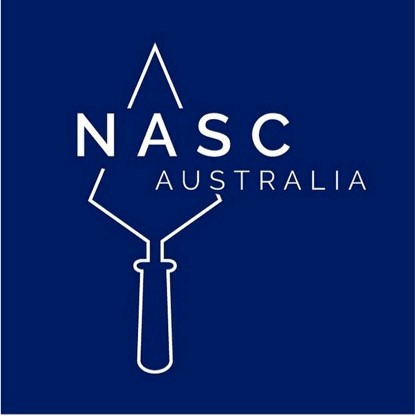
\includegraphics[width=0.4\textwidth]{figures/NASC_Fig1.jpg}%{./Pictures/mainscreen1.png}
		\caption{The updated logo for the National Archaeology Student Conference in Australia. Design credit goes to Kayla Tenielle Gourlay.}
		\label{fig:NASC_Fig1}
	\end{center}
	\vspace{-20pt}
	\vspace{1pt}
\end{wrapfigure} 

The pre-conference activities happened on the \nth{13} of August and included a guided tour of the Nicholson Museum at the University of Sydney by Dr Craig Barker and a walking excursion of the heritage area in ‘\textit{The Rocks}’ within Sydney, led by archaeologist Wayne Johnson from Sydney Harbour Foreshore Authority (SHFA). 

The morning sessions of the first day were held at the Macquarie Art Gallery and started with an acknowledgement of country by Amelia Corr of the Indigenous Studies department, on behalf of the Darug community and a welcoming address by Macquarie University Deputy Vice Chancellor, John Simons. The aim of this morning was focused on providing attendees with the opportunity to listen and engage with individuals whom have experience in excavating and networking advice followed by a Q\&A panel of our Keynote speakers and guest speaker Associate Professor Kenneth Sheedy from Macquarie University. Samantha Jones and Rodney Cross presented about their recent involvement with the ‘\textit{Australian Carsulae Archaeological Project}’ (ACAP) in excavating the ancient Roman Town of Carsulae in Umbria, Italy (220 BC–AD 250). The workshop described the cultural history of the site, as well as the surveys performed to explore the geophysical characteristics of the area.\footnote{Much thanks to Samantha Jones who helped to amend this and the previous sentence.}

\begin{figure}
	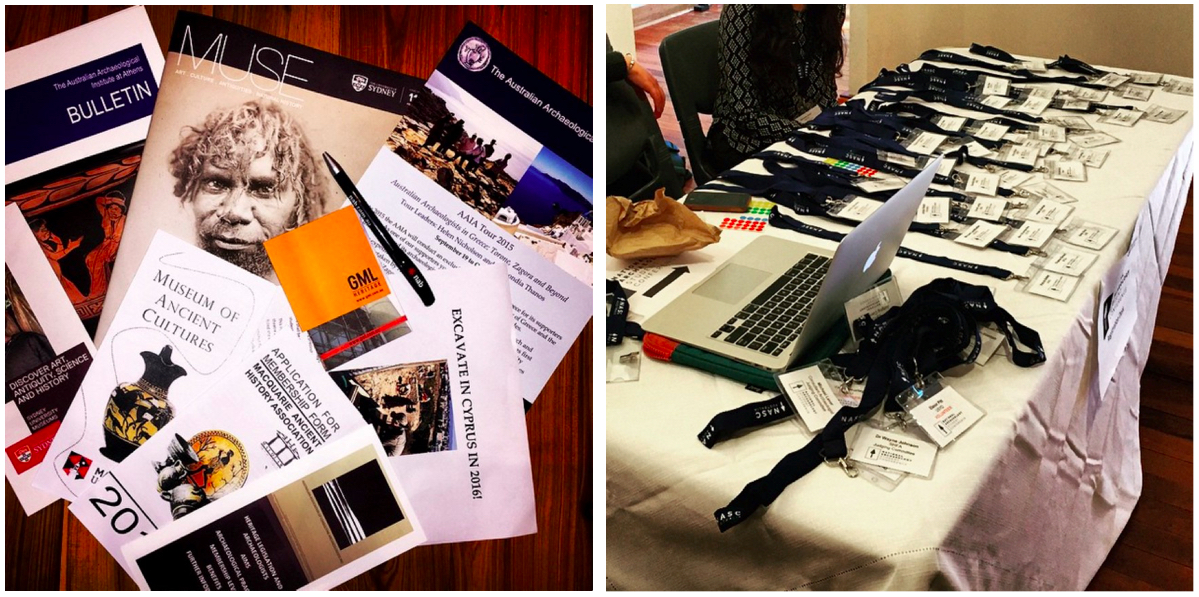
\includegraphics[width=\linewidth]{figures/NASC_Fig2}
	\centering
	\caption{(\textit{Left}) The conference bags contents. (\textit{Right}) Registration table set up for the conference including lanyards for all attendees.}
	\label{fig:NASC_Fig2}
\end{figure}

Macquarie PhD candidate, Aaron de Souza, presented ‘\textit{Making Connections: Building Networks in Archaeology}’ to the student delegates about the importance of networking in archaeological circles. This was based on his own experience whilst obtaining fieldwork and museum visits for his Egyptian archaeological research. Aaron emphasised key strategies for developing your professional network, these include asking for help from your supervisor or fellow colleagues, contacting relevant experts for research advice, talking to new people while attending conferences, selling yourself as a potential employee, and taking risks to get ahead. NASC organisers felt it was imperative that this information is provided to attendees from a PhD student to allow them to connect and understand that opportunities in archaeology are available to students. The Q\&A panel followed, where questions were asked of the panel members about their life and careers in archaeology; such as Amanda’s efforts to increase the awareness and importance of cultural heritage in South Africa, specifically at school level; Aedeen’s PhD experience and its importance as a qualification that anyone should attempt to gain and Ken’s thoughts on the job prospects for archaeologists lying within cultural heritage occupations. Audience members followed up with their own questions, allowing an informal discussion about the state of Archaeology today and the need for current students to broaden their skill set in order to be employable.

Afternoon workshops focused on providing students with an insight into practical archaeological skills. PhD candidate, Mary Hartley (MQU), presented her ‘\textit{Archaeological Illustration Experience Workshop}’ where she taught the basics and importance of technical archaeological fieldwork illustration (Fig. \ref{fig:NASC_Fig3}); not to mention her experiences in hand drawing artefacts for Macquarie’s Egyptian excavations at Thebes near Luxor. Macquarie staff members, Dr. Adela Sobotkova, Dr. Brian Ballsun-Stanton and Assoc. Prof. Shawn Ross, demonstrated a practical demo of their \textit{Federated Archaeological Information Management Systems} (FAIMS) project mobile app, which allows offline digital recording on the field. Students were given a theoretical introduction about the app’s purpose and design, followed by a practical, where the students used the app on provided tablets or on their own electronic devices. These two archaeological recording workshops complemented each other, emphasising that paper recording is still a requirement but that technology can also be integrated into field recording. After a long day of workshops, the Macquarie Staff Café hosted the student attendees for a BBQ dinner, before attending the keynote presentation by Dr. Aedeen Cremin at Macquarie’s Museum of Ancient Culture’s seminar room. Aedeen discussed her presentation ‘\textit{Peripheral Vision}’ which focussed on the idea of the Beaker “culture” and their cultural material indicator the bell-beaker. Part of her presentation discussed the limitations in defining this culture through just relying on the ceramic evidence and exploring other indicators, such as dental remains.

\begin{figure}
	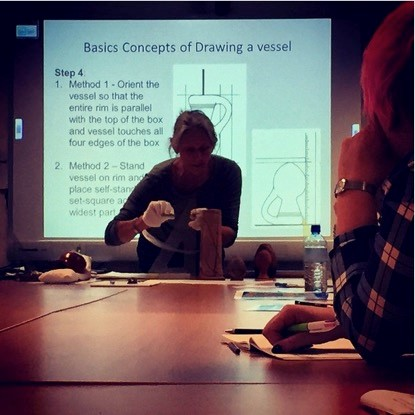
\includegraphics[width=.6\linewidth]{figures/NASC_Fig3}
	\centering
	\caption{Mary Hartley from Macquarie University whilst presenting her 'Archaeological illustration experience workshop'.}
	\label{fig:NASC_Fig3}
\end{figure}	
	
Conference proceedings over the weekend were held at the University of Sydney in the Footbridge theatre, a former theatre transformed into a 500-seat lecture space with great acoustics. The lecture hall was chosen as it provided enough room for attendees as well as a more intimate and less confronting setting for student presenters, particularly for those presenting at their first conference. Furthermore, to provide feedback to students, a panel of judges including academics and professional archaeologists evaluated presentations and posters. This was to provide valuable feedback for the students, as no doubt they would be presenting at future conferences in their academic career. Feedback from all of the judges was then sent to each presenter after the conference and prizes were also awarded for each academic level. The panel of judges included Michael Lever (Consultant Archaeologist), Dr Peter Keegan (MQU), Dr Wayne Johnson (Sydney Harbour Foreshore Authority), Dr Annie Clarke (USYD), Dr Patrick Faulkner (USYD) and keynote speaker Associate Professor Amanda Esterhuysen. 

The Saturday began with a welcoming address from the Organising Committee chairperson, Rebekah Hawkins, followed by a ‘\textit{Welcome to Country}’ by Uncle Chicka on behalf of the Cadigal community. Four sessions of research papers were conducted that day and each presentation was allocated fifteen minutes to present with five minutes for questions. Morning tea, lunch and afternoon tea were provided as part of the registration fee. Session one was chaired by Olivier Rochecouste (MQU), with three research papers; Honours students Natasha Naughton (USYD) and Francesca McMaster (USYD), along with PhD candidate, Jordan Ralph (Flinders). Session two was chaired by Sharna Katzeff (USYD), with presentations by PhD candidate Liesel Gentelli (UWA) as well as Greg Sing (USYD) and Sarah Janson (USYD). Session three was overseen by Patrick Bailey (ANU) with two Honours student presentations, Bronwyn Woff and James Donon (La Trobe) along with PhD candidate Ben Dharmendra (USYD). Session four was chaired by Kelsey Rydar (ANU), with a presentation by PhD candidate, Georgia Roberts (La Trobe) along with two undergraduate students, Chris Silvester (La Trobe) and Marc Cheeseman (UQLD). A fifth session followed for the presentation of seven research posters on display in the downstairs foyer; these included posters by Emmy Frost (La Trobe), Benjamin Bassett (MON), Harriet Donnelly \& Samantha Leggett (USYD), Georgia Burnett (MQU), Felicity Buckingham (La Trobe), Anthony Romano (La Trobe) and Georgia Roberts (La Trobe). 

Amanda ended the day’s proceedings with her keynote presentation, ‘\textit{A retro- and introspection of post-1994 archaeology in South Africa}’. This presentation examined her experience with preserving South Africa’s cultural heritage and its clash with past and present political issues involved. This included being challenged by past apartheid ideals that confronted her when trying to reach out to schools and incorporate evolution into the curriculum. Continuing, with her experiences with native burial customs and tribal belief systems and how they clash with, for example, mining companies. As a result, she elegantly demonstrated the need for archaeology students to be aware of modern political goals and both modern and past cultural beliefs of any country they wish to work in to properly respect and co-operate with the individuals of a community or region. 


\begin{figure}
	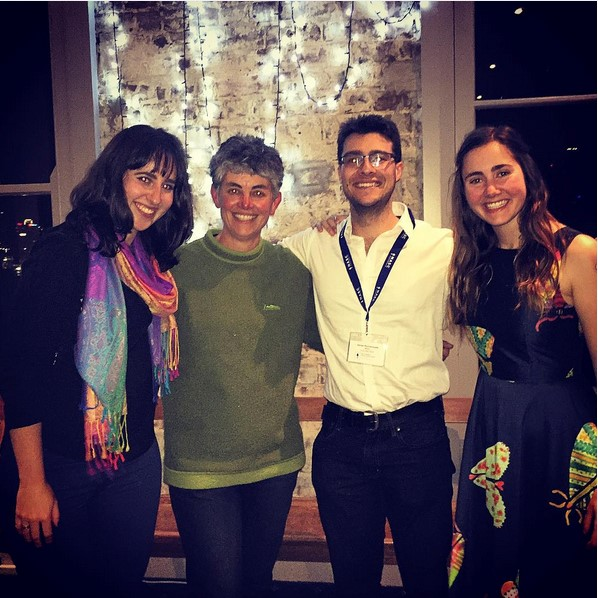
\includegraphics[width=.6\linewidth]{figures/NASC_Fig4}
	\centering
	\caption{Sharna Katzeff (Vice Chairperson), Assoc. Prof. Amanda Estherhuysen, Olivier Rochecouste (Treasurer) and Rebekah Hawkins (Chairperson) at the closing conference dinner.}
	\label{fig:NASC_Fig4}
\end{figure}


Sunday the \nth{16} of August was the last day of conference proceedings. Session six was chaired by Ada Dinckal (La Trobe) and was a unique session that had students present their recent fieldwork experiences. The conference is run by students for students and the aim of this session was to provide students an opportunity to hear about excavations that are happening around the world and hear about fieldwork. This was particularly aimed at the lack of fieldwork opportunities in Australia compared to elsewhere, like Europe, the Levant or the Middle East. Since this was a more informal presentation compared to the research presentations, students were given a ten-minute slot to present their fieldwork experience and questions followed. This session included presentations by Brenan Dew (MQU), Coral Hardwick \& Eli Gentzakis (MQU), Margot Murray (UNIMELB), Sharna Katzeff (USYD), Charlotte Kowalski (USYD) and Hannah Morris (USYD). Research sessions then continued and session seven was chaired by Melissa Bendell (UNE) with four presentations, Masters candidate, Michael Leadbetter (USYD), Honours student Elanor Pitt (USYD) as well as PhD candidates Jacob Heywood (UMELB) and Charles Barnett (MQU). Session eight was chaired by Benjamin Bassett (MON), featuring a presentation by honours student Ané van der Walt (USYD) and two collaborative presentations by students of ANU; Kelsey Rydar, Simon Williams, Sean Sheehan, Melandri Vlok, Lucy Blackam and Marni Booth. Session nine was overseen by Georgia Roberts (La Trobe), containing presentations by Honours student Adam Valka (La Trobe) and PhD candidates Olivier Rochecouste (MQU) and Amy Way (USYD). The tenth and final session, chaired by Rebekah Hawkins (USYD), featured Honours student Rebecca Morris (USYD) and Undergraduate student Colin Randall (USYD). 

The conference judges were asked to give general feedback to the students before closing the conference. The judges felt that the presenters portrayed ideas and case studies which were rich and of a world class conference standard. Furthermore, they encouraged and emphasised presentation skills such as engaging the audience and limiting words on a PowerPoint. 

The conference closing night dinner was held at the Toxteth Hote. Before the dinner started, awards were presented for each student level presentation, poster and excavation experience presentation. The winners of each category were Chris Silvester (Undergraduate), Ané van der Walt (Honours), Michael Leadbetter (Masters), Georgia Roberts (PhD), Benjamin Bassett (Poster) and Hannah Morris (Excavation). The ‘Bruce G. Trigger Award for Archaeological Thought’ award was also given to the presentation that showed originality, flexibility and a critical understanding of archaeological thought. It was awarded to Michael Leadbetter (USYD) for his presentation ‘Cities Across the South-China Seas’, with honourable mentions going to Francesca McMaster (USYD) and Olivier Rochecouste (MQU).

\begin{figure}
	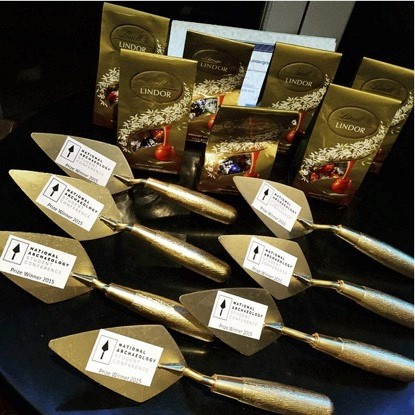
\includegraphics[width=.6\linewidth]{figures/NASC_Fig5}
	\centering
	\caption{Each winner received a certificate, chocolates and a unique NASC gift; a golden trowel.}
	\label{fig:NASC_Fig5}
\end{figure}

Deciding where the next NASC in Australia would be, was discussed in a forum during the lunch break on Saturday \nth{15}. Interested students from a range of universities were invited to listen to the 2015 Core Organising Committee’s experience organising the conference and had the opportunity to ask them questions. This was also used as a time to judge the interest from the student body to continue NASC. The fact that NASC is not associated to any particular university is both a benefit and disadvantage. It’s beneficial as it allows students from a range of universities to hopefully gain experience in holding a conference, and with each new university, their focus in archaeology may differ slightly and as a result Keynote speakers and judges that are invited will differ each year. This not only is beneficial to the students organising the conference, but also to the attendees as it exposes them to different fields, thoughts and practices within archaeology. However, it does mean that each year a new organising committee takes charge in organising the conference, preferably one that is composed of a new group of willing, enthusiastic and committed students who are prepared to take on the conference for the next year. It also means that dates and venues change each year depending on the organisation capabilities and location of the organising committee. 

Even though there are limitations and challenges in running a student conference, organised by students, the benefits outweigh all the costs. NASC allows students to present in a welcoming environment and practice their presentation skills before presenting what will be numerous papers in their academic careers. Furthermore, the last two committees have chosen to run NASC with no parallel sessions. There are a number of reasons for this decision; firstly it provides students a respectful audience that will listen to any and all presentations that have been prepared for the conference. Additionally, it’s a student conference and encouraging undergraduate students to attend is imperative to facilitate its future. By listening to all presentations, students can appreciate the complexity of this discipline and listen to the wide range of archaeological topics, regions, techniques and skills it has to offer. We can only hope that those students who were looking for some inspiration found it during their time at NASC. Having everyone present together, with such a broad array of research topics, there was a considerable effort by the organising team to try and create themes for each session, or links between presentations where possible. Last but not least, conferences are a time to network and realistically the students at the conference this year, will be at conferences together in the future for a few decades to come. Why not let them learn how to appreciate and engage in archaeology now, before academic rigour means they will be attending conferences that are only pertinent to their own research? 

After evaluating many proposals, the \emph{University of Western Australia}, Perth has been selected to host NASC 2016. NASC invites students nationally and internationally to attend the conference and if you would like to stay informed with its upcoming dates and venues, follow our \href{https://www.facebook.com/nascaustralia}{Facebook} page or \href{http://www.nascaustralia.com/}{website} for further details.

	\SetBlockThreshold{1} 
	\blockquote{\textit{Thanks to our sponsors; Macquarie University, The University of Sydney, National Australia Bank (NAB), GML Heritage, Australian Association of Consulting Archaeologists INC (AACAI), Comber Consultants, Australia Archaeology Institute at Athens (AAIA), The Museum of Applied Arts \& Sciences (MAAS), The Nicholson Museum (USYD), Museum of Ancient Cultures (MQU), The USYD Archaeology Society (ArchSoc), The Museum Appreciation Society of Macquarie (MAS) and the Macquarie Ancient History Association (MAHA).}}



	\label{NASC:lastpage}
	%----------------------------------------------------------------------------------------
\closingarticle
